\begin{table}
    \def\widthspark{120pt}
    \centering
    \caption[Acoustic material definitions]{Common acoustic absorption coefficients with ranges (low-high) of $\alpha$ absorption characteristics across the frequency bands for those material types. It should be noted that these are regressions and averages of generally adopted materials and existing measurement tables; realistic or surveying acoustic simulations should adopt absorption measurements of real materials.}
    \begin{tabular}{lll}
    \toprule
    \textbf{Material}                  & \textbf{Low $\alpha$}                                                              & \textbf{High $\alpha$}                                                               \\ \midrule
    Glass and glazing                  & 
\includegraphics[width=\widthspark]{sparklines/glass and glazing_low}               & 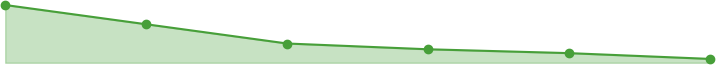
\includegraphics[width=\widthspark]{sparklines/glass and glazing_high}               \\ 
    Masonry walls                      & 
\includegraphics[width=\widthspark]{sparklines/masonry walls_low}                   & 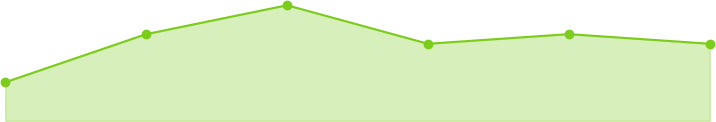
\includegraphics[width=\widthspark]{sparklines/masonry walls_high}                   \\ 
    Stud-work \& lightweight walls     & 
\includegraphics[width=\widthspark]{sparklines/studwork and lightweight walls_low}  & 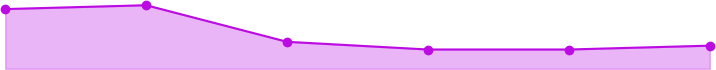
\includegraphics[width=\widthspark]{sparklines/studwork and lightweight walls_high}  \\ 
    Wood \& wood panelling             & 
\includegraphics[width=\widthspark]{sparklines/wood and wood panelling_low}         & 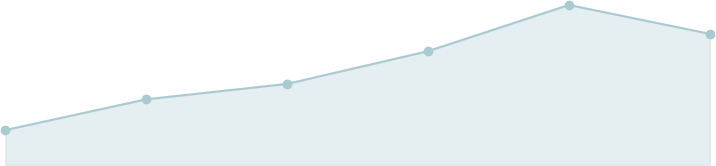
\includegraphics[width=\widthspark]{sparklines/wood and wood panelling_high}         \\ 
    Floors                             & 
\includegraphics[width=\widthspark]{sparklines/floors_low}                          & 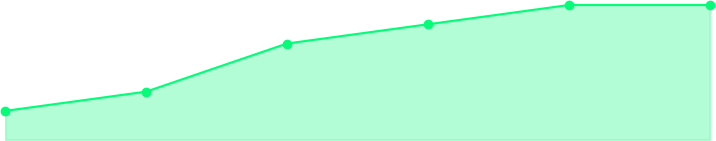
\includegraphics[width=\widthspark]{sparklines/floors_high}                          \\ 
    Panels \& doors                    & 
\includegraphics[width=\widthspark]{sparklines/panels and doors_low}                & 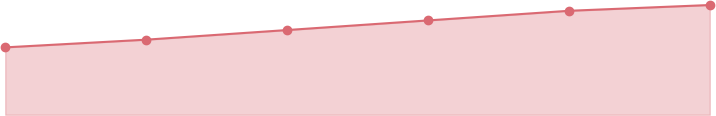
\includegraphics[width=\widthspark]{sparklines/panels and doors_high}                \\ 
    Other                              & 
\includegraphics[width=\widthspark]{sparklines/other_low}                           & 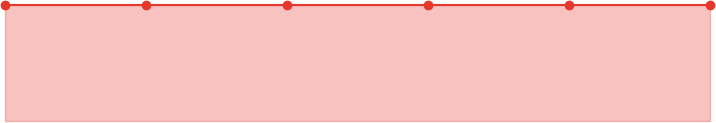
\includegraphics[width=\widthspark]{sparklines/other_high}                           \\ 
    Wall treatments \& construction    & 
\includegraphics[width=\widthspark]{sparklines/wall treatments & constructions_low} & 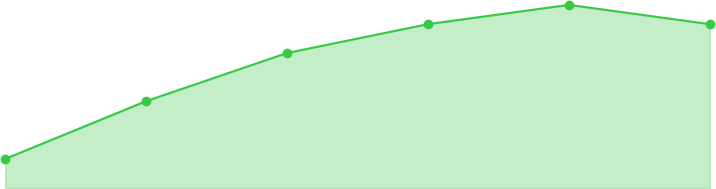
\includegraphics[width=\widthspark]{sparklines/wall treatments & constructions_high} \\ 
    Ceilings                           & 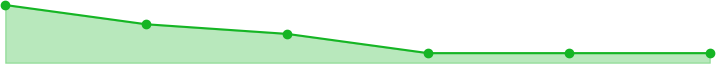
\includegraphics[width=\widthspark]{sparklines/ceilings_low}                        & 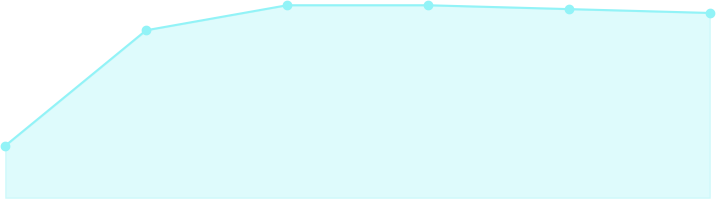
\includegraphics[width=\widthspark]{sparklines/ceilings_high}                        \\ 
    Mineral wool \& foams              & 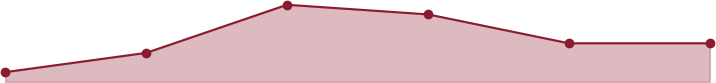
\includegraphics[width=\widthspark]{sparklines/mineral wool and foams_low}          & 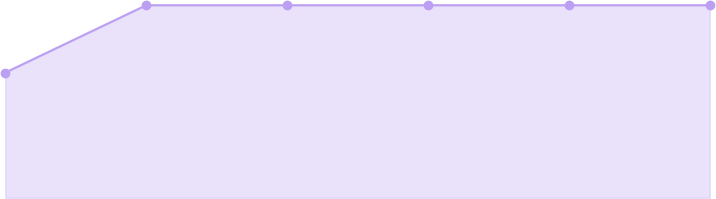
\includegraphics[width=\widthspark]{sparklines/mineral wool and foams_high}          \\ 
    Audience \& seating                & 
\includegraphics[width=\widthspark]{sparklines/audience and seating_low}            & 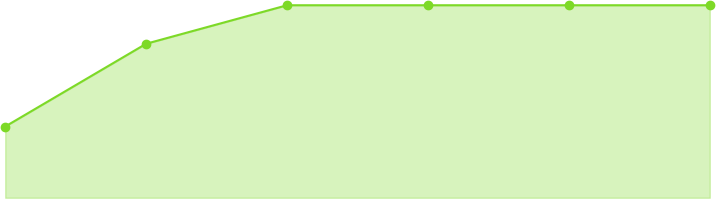
\includegraphics[width=\widthspark]{sparklines/audience and seating_high}            \\ 
    \bottomrule
    \end{tabular}\label{tab:absorption-coeffs}
\end{table}